\section{Features}

\subsection{User interface language}
\label{sec:features:language-selector}
Germinate fully supports internationalization. This means that the interface can be translated into any number of languages. By default, Germinate is distributed in English. Depending on the configuration of Germinate, other languages might be available. You can switch between them by selecting a language from the first dropdown box shown in Figure \ref{fig:overview:home}C.

\subsection{Groups}
In Germinate we define the concept of a group to be an arbitrary grouping of database items of a certain type. Germinate supports groups of \textit{accessions}, \textit{markers} and \textit{locations}. These groups can be pre-created by an administrator or user-defined, which means that you can create your own groups (assuming user authentication is enabled).

The purpose of these groups becomes clear once you start exporting data. All types of data can either be exported for the whole dataset or the data can be subset into smaller chunks by selecting a single or a selection of groups. The exported data will then contain information about the selected groups only.

An example of this is shown in Figure \ref{fig:features:group-subselection} where we selected a group of accessions (192 out of 2000 accessions) and a group containing a single marker (out of 5000). The resulting data file will consequently contain at most 192 rows and at most a single column of data (it may contain less, if the selected database items are not actually part of the selected dataset).

\begin{figure}
	\centering
	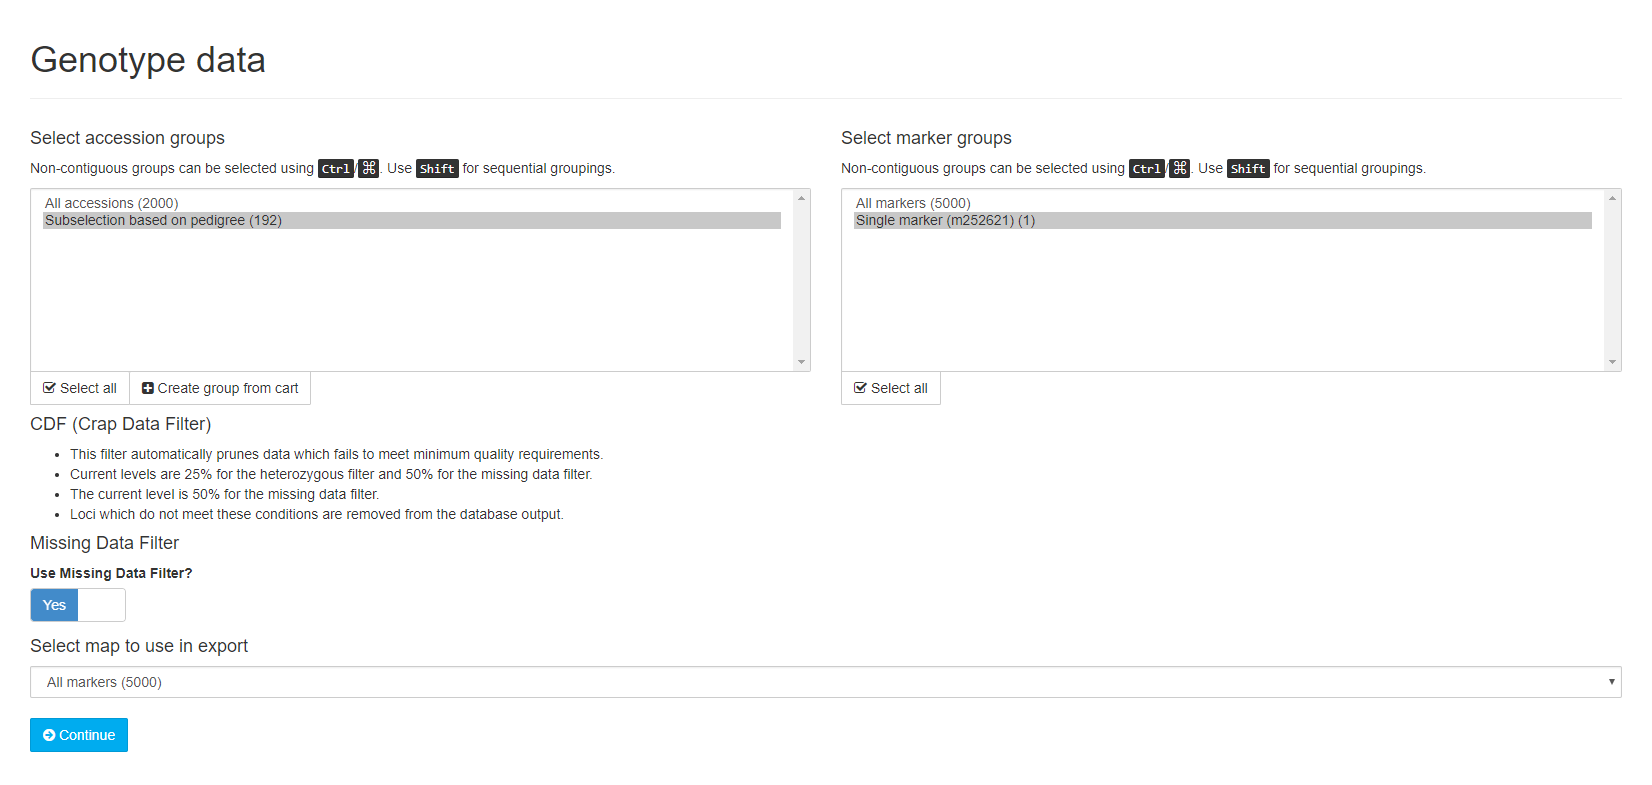
\includegraphics[width=0.85\linewidth]{img/features/group-subselection.png}
	\caption{Example of the group sub-selection feature: You can select both accession and marker groups during the genotypic data export process to subset the dataset.}
	\label{fig:features:group-subselection}
\end{figure}

\subsubsection{Creating a group}
\textit{This section is only applicable if the Germinate instance you are using has user authentication enabled.}\\
\\
In addition to using the predefined groups, you can create new groups of your own. There are multiple ways in which you can create a new group and add items to it. One option is to go to the \textit{Groups} page of Germinate. This page shows you all the existing groups in a table and upon selection, shows you its group members. Figure \ref{fig:features:groups-page} shows you an example of what the groups page can look like. In this example, Germinate contains 118 different groups that the current user can see. New groups can be added and existing ones deleted by pressing the buttons below the groups table (Figure \ref{fig:features:groups-page}A). Deleting a group requires you to select the checkbox in the corresponding table row as well as to have sufficient permissions to do so. When creating a new group you will be asked to select the group type and to decide on a name for the group. When you do so, the group will be associated with your user account.

Once this is done, the group will be created and Germinate will automatically select it and show the group members table (empty at this point) below the groups table. You can now manipulate the group itself by adding and removing members using the buttons below the table as shown in Figure \ref{fig:features:groups-page}C. \todo{More info here}

Groups can be made public so that other users have the option to use them as well. If you decide to make your group public, toggle the switch button shown in Figure \ref{fig:features:groups-page}B.

\begin{figure}
	\centering
	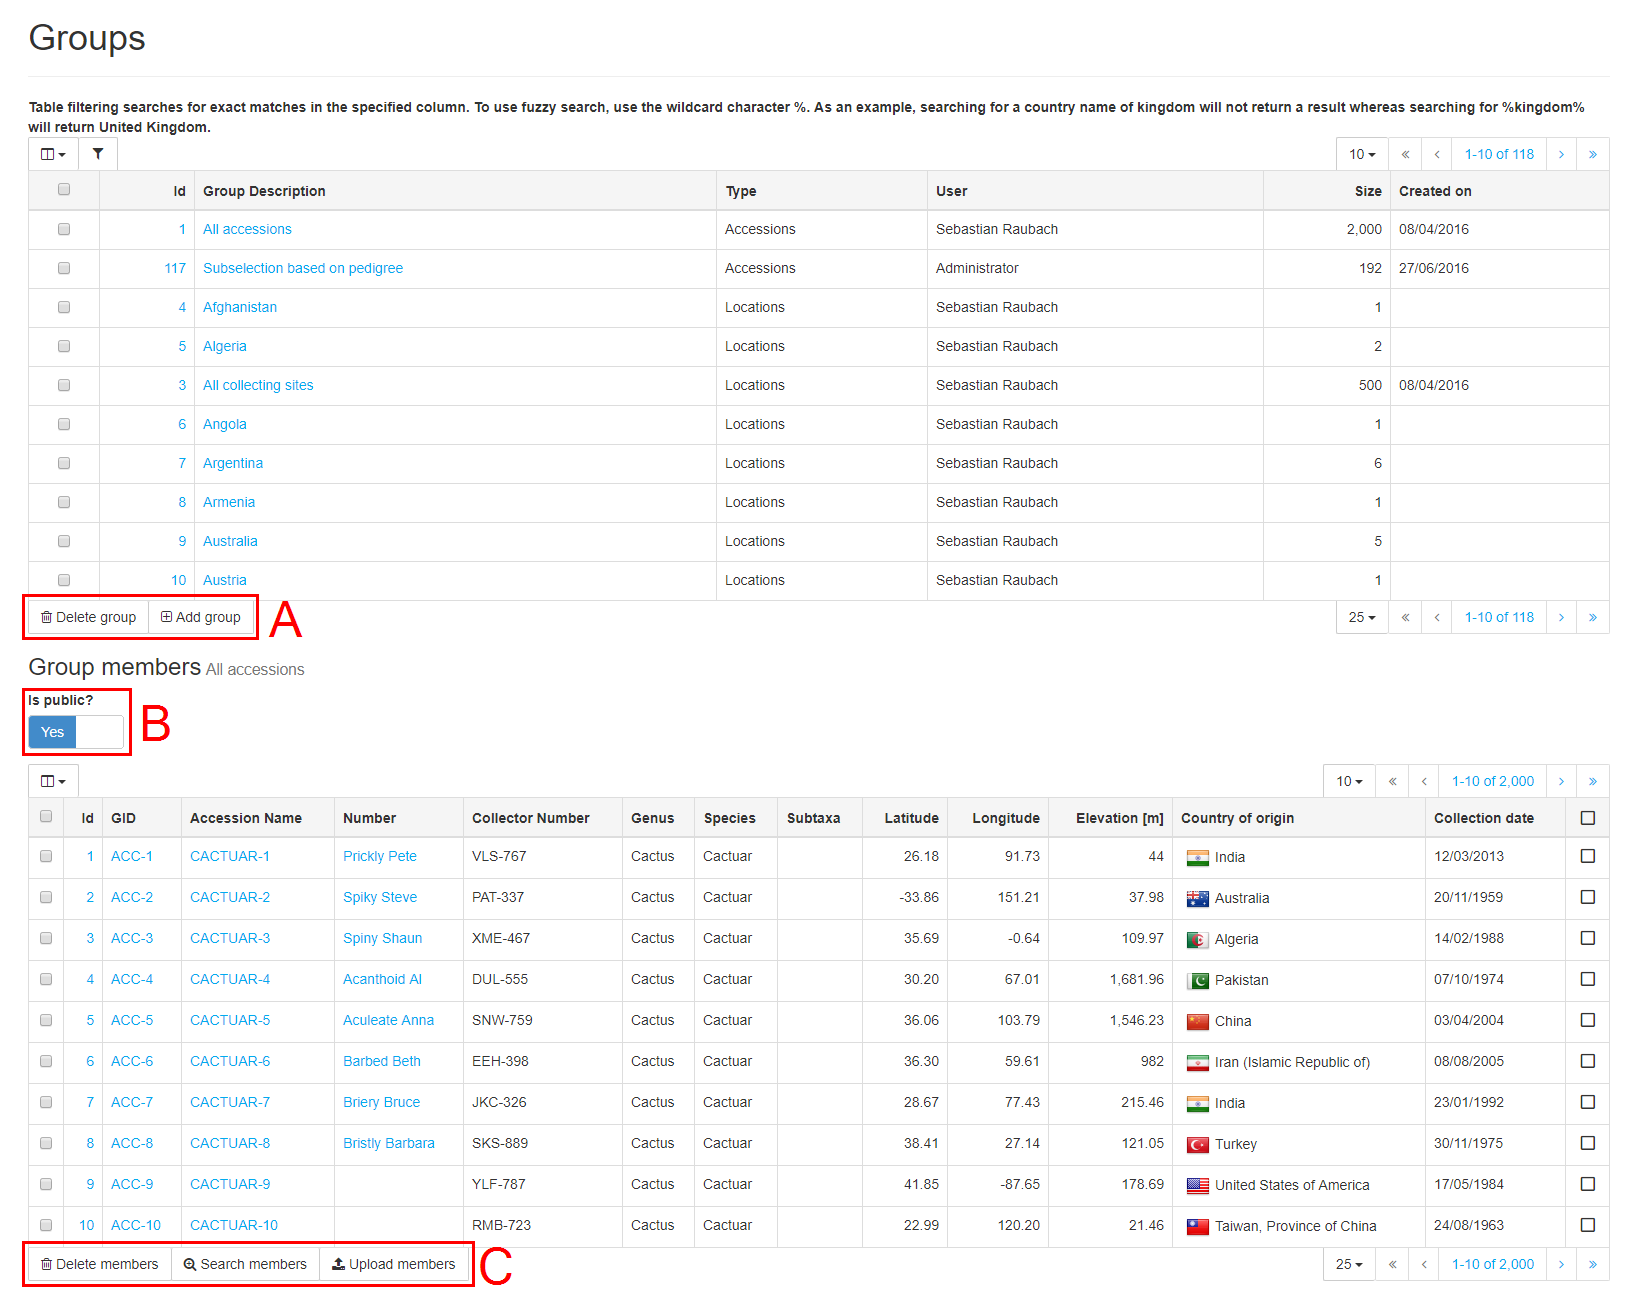
\includegraphics[width=0.85\linewidth]{img/features/groups-page.png}
	\caption{The groups page has many ways in which you can manipulate existing groups and create new groups. The top table shows all the groups that are visible to the current user. The bottom table shows the members of this group, \ie the database items that are part of it; depending on the type of the group, this can be either \textit{accessions}, \textit{markers} or \textit{locations}. (A) Groups can be added and deleted by clicking on the buttons located just below the groups table. Deleting groups requires the checkbox of the corresponding table row to be selected. (B) The group visibility can be changed by toggling this switch. A public group is visible to every user whereas an invisible group is only visible to the owner. (C) Group members can be added and removed by clicking on the buttons below the group member table.}
	\label{fig:features:groups-page}
\end{figure}

\subsubsection{Marked item lists}
\label{sec:features:marked-items}

Another useful feature of Germinate is the concept of \textit{marked item lists}. A marked item is either an accession, a marker or a location that is of interest to the user. While you are browsing the page, a lot of the tables will have a checkbox column as the last column which you can use to mark certain items. Germinate will keep track of these items for you.

To see how many items you currently have marked, you can click on the menu item as shown in Figure \ref{fig:features:marked-items-dropdown} or go directly to the marked item lists page that is shown in Figure \ref{fig:features:marked-items-page}.

Once you have marked all the items that you are interested in, you can create a group of these items and use them to export data against them. To create a group, you can either go to the marked item lists page or by clicking on the header of the checkbox column and selecting "Create group from selection" (see Figure \ref{fig:features:marked-items-context}).

\begin{figure}
	\centering
	\begin{subfigure}[b]{0.2\linewidth}
		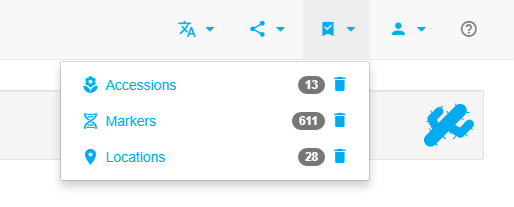
\includegraphics[width=1\linewidth]{img/features/item-list-dropdown.png}
		\caption{Dropdown}
		\label{fig:features:marked-items-dropdown}
	\end{subfigure}
	\begin{subfigure}[b]{0.58\linewidth}
		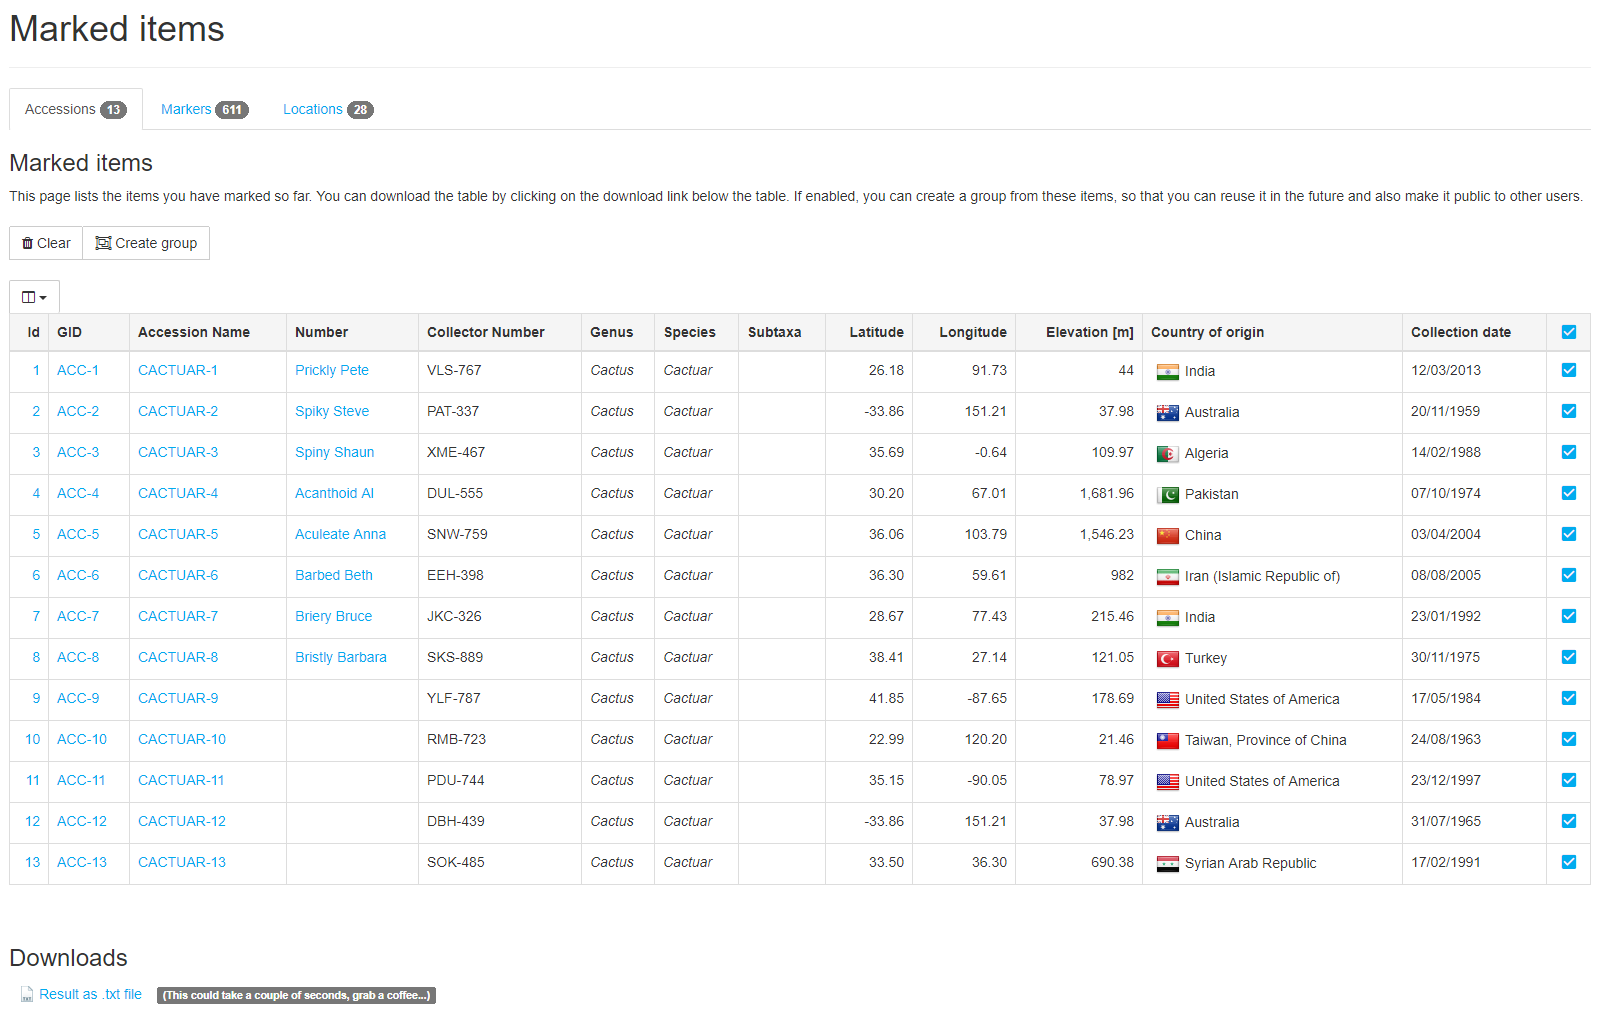
\includegraphics[width=1\linewidth]{img/features/item-list-page.png}
		\caption{Page}
		\label{fig:features:marked-items-page}
	\end{subfigure}
	\begin{subfigure}[b]{0.2\linewidth}
		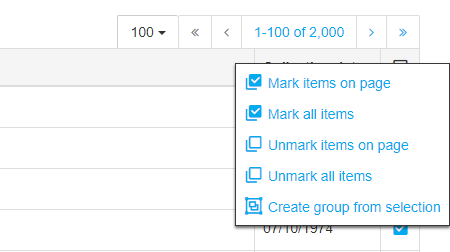
\includegraphics[width=1\linewidth]{img/features/item-list-context-create-group.png}
		\caption{Context menu}
		\label{fig:features:marked-items-context}
	\end{subfigure}
	\caption{The marked item lists keep track of items of interest. (a) }
\end{figure}


\subsection{Help}
\label{sec:features:help}